% =====================================================================
%  Evictable Vector Commitments for Verifiable LLM Inference
%  under KV-Cache Eviction  --  FULL DRAFT (Parts 1-3 merged + skeleton)
%
%  Compiles standalone (article + amsthm + graphicx). Requires the file
%  evictvc_fig1.png in the project directory (the audit-proof-size plot).
%
%  Technical core (Sections 3-8) is complete and proof-checked.
%  Sections 1, 2, 9, 10 are drafts/skeletons to be filled in; search for
%  "TODO" to find the spots that still need your input or citations.
%
%  For IACR CiC: replace the preamble down to \begin{document} with the
%  iacrcc class + front matter, and keep the theorem/macro block below.
% =====================================================================
\documentclass[11pt]{article}

\usepackage[utf8]{inputenc}
\usepackage[T1]{fontenc}
\usepackage{amsmath,amssymb,amsthm,mathtools}
\usepackage{xspace}
\usepackage{enumitem}
\usepackage{array}
\usepackage{booktabs}
\usepackage{graphicx}
\usepackage[margin=1in]{geometry}
\usepackage[colorlinks=true,linkcolor=blue,citecolor=blue,urlcolor=blue]{hyperref}

% ---------- theorem environments ----------
\theoremstyle{definition}
\newtheorem{definition}{Definition}[section]
\newtheorem{construction}{Construction}[section]
\newtheorem{assumption}{Assumption}[section]
\theoremstyle{plain}
\newtheorem{theorem}{Theorem}[section]
\newtheorem{lemma}{Lemma}[section]
\newtheorem{corollary}{Corollary}[section]
\theoremstyle{remark}
\newtheorem{remark}{Remark}[section]

% ---------- notation macros ----------
\newcommand{\secpar}{\lambda}
\newcommand{\negl}{\mathsf{negl}}
\newcommand{\PPT}{\mathrm{PPT}}
\newcommand{\bit}{\{0,1\}}
\newcommand{\sample}{\xleftarrow{\;\$\;}}
\newcommand{\defeq}{\vcentcolon=}
\newcommand{\concat}{\,\|\,}

\newcommand{\Setup}{\mathsf{Setup}}
\newcommand{\Commit}{\mathsf{Commit}}
\newcommand{\Open}{\mathsf{Open}}
\newcommand{\Vfy}{\mathsf{Verify}}
\newcommand{\Update}{\mathsf{Update}}
\newcommand{\Evict}{\mathsf{Evict}}
\newcommand{\VfyEvict}{\mathsf{VerifyEvict}}
\newcommand{\Rem}{\mathsf{Rem}}

\newcommand{\pp}{\mathsf{pp}}
\newcommand{\aux}{\mathsf{st}}
\newcommand{\Pol}{\mathsf{Pol}}
\newcommand{\HistDig}{\mathsf{HistDig}}
\newcommand{\Adv}{\mathsf{Adv}}
\newcommand{\Exp}{\mathsf{Exp}}
\newcommand{\Val}{\mathrm{val}}
\newcommand{\Sc}{\mathrm{sc}}
\newcommand{\Cval}{C_{\Val}}
\newcommand{\Csc}{C_{\Sc}}
\newcommand{\Live}{\Lambda}
\newcommand{\Evicted}{E}
\newcommand{\A}{\mathcal{A}}
\newcommand{\B}{\mathcal{B}}
\newcommand{\Vsp}{\mathcal{V}}
\newcommand{\Ssp}{\mathcal{S}}
\newcommand{\Tsp}{\mathcal{T}}
\newcommand{\hash}{\mathsf{H}}
\newcommand{\VC}{\mathsf{VC}}
\newcommand{\Log}{\mathcal{L}}
\newcommand{\GG}{\mathbb{G}}
\newcommand{\FF}{\mathbb{F}}
\newcommand{\gone}[1]{\left[#1\right]_{1}}
\newcommand{\gtwo}[1]{\left[#1\right]_{2}}
\newcommand{\gtt}[1]{\left[#1\right]_{T}}
\newcommand{\dom}{\mathbb{D}}
\newcommand{\lag}{\ell}
\newcommand{\srs}{\mathsf{srs}}
\newcommand{\nsdh}{n\text{-}\mathsf{SDH}}
\newcommand{\Zpol}{Z}
\newcommand{\rpol}{r}
\newcommand{\posbind}{\mathsf{pos\text{-}bind}}
\newcommand{\evsnd}{\mathsf{ev\text{-}snd}}
\newcommand{\polbind}{\mathsf{pol\text{-}bind}}
\newcommand{\histte}{\mathsf{hist\text{-}te}}
\newcommand{\collres}{\mathsf{cr}}

\title{Evictable Vector Commitments:\\
       Verifiable LLM Inference under KV-Cache Eviction}
\author{Liu Kefan\thanks{Nanyang Technological University, Singapore.
        Correspondence: \texttt{<your-email>}.}}
\date{\today}

\begin{document}
\maketitle

\begin{abstract}
Verifiable LLM inference lets a client check that a model was executed
faithfully on its input. Existing schemes commit to the entire retained
activation state and therefore cannot account for \emph{KV-cache eviction}:
the permanent deletion of token key/value states performed by streaming cache
compressors such as StreamingLLM, H2O, and SnapKV. We introduce
\emph{evictable vector commitments} (EvictVC), a commitment primitive whose
committed positions can be permanently evicted under a public eviction policy
while a tamper-evident history of every deletion is maintained. We formalize
the primitive with a syntax and three game-based security notions---eviction
soundness, policy-binding, and history tamper-evidence---and give a
construction from KZG polynomial commitments in which an eviction is a single
group operation independent of the cache size, an audit proof for an arbitrary
set of positions is a single group element, and all opening proofs are
maintainable in quasi-linear time via the Feist--Khovratovich technique. We
prove security under the $\nsdh$ assumption and the collision resistance of a
hash function. A prototype over BLS12-381 confirms the asymptotics: eviction and
commitment updates cost ${\approx}\,135\,\mu\mathrm{s}$ irrespective of cache
length up to $2^{16}$, verification is two pairings
(${\approx}\,2.6\,\mathrm{ms}$), and audit proofs are $48$ bytes regardless of
how many positions are audited.
\end{abstract}

% =====================================================================
\section{Introduction}\label{sec:intro}
% =====================================================================

Delegated large-language-model inference increasingly runs on servers a client
does not control. \emph{Verifiable inference} addresses the resulting trust gap
by having the server commit to its computation and prove that the claimed output
follows from a faithful execution. A common ingredient is a commitment to the
model's intermediate state, against which the server later opens individual
values to answer audit challenges.

A central object of that state is the \emph{key/value (KV) cache}: the stored
attention keys and values for every past token. The cache grows linearly with
context length, so production systems compress it. Streaming compressors such as
StreamingLLM, H2O, and SnapKV do so by \emph{permanently evicting} the
key/value states of tokens deemed unimportant under an attention-based policy.
Eviction is destructive: the evicted state is gone and can never be opened
again.

This destructiveness breaks existing verifiable-inference commitments, which
assume the committed state remains fully present and openable. Three problems
arise simultaneously. First, the commitment must be able to \emph{shrink}: an
evicted position can no longer be claimed to hold a value. Second, eviction must
be \emph{policy-bound}: a malicious server must not be able to drop an
inconvenient (e.g.\ high-attention) position while claiming it followed the
compressor's policy. Third, the server must not be able to \emph{rewrite history}:
the record of which positions were evicted, and with what values, must be
immutable so that an auditor can reconstruct and check the entire compression
trajectory.

We resolve all three with \emph{evictable vector commitments}. An EvictVC commits
jointly to a value vector and a per-position score (attention) vector. It
supports the usual openings and homomorphic updates, and adds an $\Evict$
operation that (i) removes a position from the live value commitment in a single
group operation, (ii) is accepted only if the position's committed score
satisfies the public eviction policy, and (iii) appends the removed record to a
tamper-evident hash-chain history. Audits remain cheap: a proof for an arbitrary
set of live positions is a single group element, and all opening proofs are
maintainable in quasi-linear total time.

\paragraph{Contributions.}
\begin{itemize}[leftmargin=1.4em,itemsep=2pt]
  \item \textbf{A model.} We give a syntax for evictable vector commitments and
        three game-based security notions---\emph{eviction soundness},
        \emph{policy-binding}, and \emph{history tamper-evidence}
        (Sections~\ref{sec:syntax}--\ref{sec:secmodel}).
  \item \textbf{A construction.} We instantiate the primitive from KZG
        polynomial commitments over roots of unity ($\Pi_{\mathsf{KZG}}$,
        Sections~\ref{sec:kzgvc}--\ref{sec:construction}): eviction and updates
        are $O(1)$, audit proofs for any position set are a single group
        element, and all opening proofs are produced in $O(n\log n)$ via the
        Feist--Khovratovich technique.
  \item \textbf{Security proofs.} We give tight reductions: eviction soundness
        and policy-binding reduce to position binding of the KZG vector
        commitment, hence to $\nsdh$; history tamper-evidence reduces to
        collision resistance (Section~\ref{sec:proofs}).
  \item \textbf{A prototype.} A Python reference and a Rust/arkworks backend over
        BLS12-381 validate the design: eviction costs ${\approx}\,135\,\mu s$
        independent of cache size up to $2^{16}$, audit proofs are $48$ bytes
        versus linearly growing Merkle multiproofs, and Feist--Khovratovich makes
        whole-cache proof generation practical (Section~\ref{sec:eval}).
\end{itemize}

\paragraph{Organization.}
Section~\ref{sec:related} surveys related work. Sections~\ref{sec:prelim}--\ref{sec:secmodel}
develop the model. Sections~\ref{sec:kzgvc}--\ref{sec:construction} give the
construction and Section~\ref{sec:proofs} its security proofs.
Section~\ref{sec:eval} reports the evaluation and Section~\ref{sec:conc}
concludes.

% =====================================================================
\section{Related Work}\label{sec:related}
% =====================================================================

\paragraph{Verifiable and accountable LLM inference.}
The strongest guarantee is a zero-knowledge proof of the forward pass:
zkLLM~\cite{zkllm} is the first zero-knowledge argument tailored to LLMs, proving
an entire $13$-billion-parameter inference in about fifteen minutes with a proof
under $200$\,kB while keeping the model parameters hidden, via a custom lookup
argument for the non-arithmetic tensor operations. Such proofs are sound but
impose orders-of-magnitude prover overhead. A lighter line trades cryptographic
soundness for empirical or economic guarantees: VeriLLM~\cite{verillm} commits to
sampled activations with Merkle trees and re-executes roughly $1\%$ of the
computation under a one-honest-verifier assumption, deterring lazy verification
with a peer-prediction incentive, while SVIP~\cite{svip} and
TopLoc~\cite{toploc} detect deviation through lightweight activation fingerprints
and locality-sensitive hashing. A feature common to all of these is that the
prover commits to the \emph{retained} computation---activations or transcripts
that remain available to be opened or re-run. None models the \emph{permanent
deletion} of committed state, which is precisely what streaming cache compression
performs and what EvictVC targets. Moreover, the Merkle-tree commitments several
of these systems use yield audit proofs that grow with the number of checked
positions, whereas EvictVC's subvector audits are constant-size and aggregatable
(Section~\ref{sec:eval}).

\paragraph{Vector commitments.}
Vector commitments with position binding were formalized by Catalano and
Fiore~\cite{cf13}; subsequent work added single-element subvector openings and
cross-commitment aggregation~\cite{tomescu} as well as efficient local updates.
EvictVC extends this lineage with a deletion-style, policy-checked eviction
operation and an append-only, tamper-evident history, while reusing
single-element subvector openings to make batch audits constant-size.

\paragraph{KV-cache compression.}
Streaming cache compressors permanently evict the key/value states of
low-importance tokens to bound memory. StreamingLLM~\cite{streamingllm} keeps
``attention-sink'' and recent tokens under a positional window; H2O~\cite{h2o}
scores tokens by cumulative attention and retains the ``heavy hitters'';
SnapKV~\cite{snapkv} selects clustered important tokens from a prefill
observation window. In each case the unselected token states are removed from
memory and become permanently inaccessible---the destructive operation our
primitive must accommodate---and the threshold/score structure of these policies
is exactly the policy predicate that EvictVC binds. These works optimize output
quality and memory; they provide no verifiability, the orthogonal axis we add.

\paragraph{Amortized KZG proofs.}
The Feist--Khovratovich technique~\cite{fk} computes all evaluation proofs of a
KZG commitment in quasi-linear total time rather than recomputing each in
isolation. We apply it (Section~\ref{sec:eval}) so that opening proofs for the
entire, possibly-evicted cache can be produced and maintained efficiently.

% =====================================================================
\section{Preliminaries and Building Blocks}\label{sec:prelim}
% =====================================================================

\paragraph{Notation.}
We write $\secpar$ for the security parameter and $1^\secpar$ for its unary
encoding. A function is \emph{negligible}, written $\negl(\secpar)$, if it
vanishes faster than every inverse polynomial. $\PPT$ abbreviates probabilistic
polynomial time. For $n\in\mathbb{N}$ we write $[n]=\{1,\dots,n\}$. We write
$x\sample X$ for sampling $x$ uniformly from a finite set $X$. All algorithms
implicitly take $\pp$ as input once it is fixed. Concatenation of bit strings is
denoted $\concat$, and $\langle\cdot\rangle$ denotes an unambiguous (prefix-free)
encoding into $\bit^{*}$.

\paragraph{Bilinear groups.}
For the concrete instantiation we use a Type-III bilinear group
$\mathsf{bgp}=(\GG_1,\GG_2,\GG_T,e,g_1,g_2,p)$ of prime order $p$, where
$e:\GG_1\times\GG_2\to\GG_T$ is a non-degenerate efficiently computable pairing.
For $x\in\FF_p$ we write $\gone{x}\defeq x\cdot g_1$, $\gtwo{x}\defeq x\cdot g_2$,
$\gtt{x}\defeq x\cdot e(g_1,g_2)$, so that $e(\gone{a},\gtwo{b})=\gtt{ab}$. The
abstract syntax of Section~\ref{sec:syntax} is group-agnostic.

\subsection{Vector commitments with updates}

\begin{definition}[Vector commitment]\label{def:vc}
A \emph{vector commitment} over message space $\Vsp$ is a tuple of $\PPT$
algorithms $\VC=(\VC.\Setup,\VC.\Commit,\VC.\Open,\VC.\Vfy,\VC.\Update)$:
\begin{itemize}[leftmargin=1.4em,itemsep=2pt]
  \item $\VC.\Setup(1^\secpar,1^n)\to\pp$ outputs public parameters for vectors
        of length $n$.
  \item $\VC.\Commit(\pp,\mathbf{m})\to(C,\aux)$ commits to
        $\mathbf{m}\in\Vsp^{\,n}$, returning a commitment $C$ and committer state
        $\aux$.
  \item $\VC.\Open(\pp,\aux,S)\to\pi$ produces a proof for the entries indexed by
        $S\subseteq[n]$.
  \item $\VC.\Vfy(\pp,C,S,\{m_i\}_{i\in S},\pi)\to\bit$ verifies the claimed
        entries against $C$.
  \item $\VC.\Update(\pp,C,i,\delta)\to C'$ deterministically updates $C$ to the
        commitment of the vector with $m_i$ replaced by $m_i+\delta$.
\end{itemize}
We write $\Rem(\pp,C,i,m)\defeq\VC.\Update(\pp,C,i,-m)$ for the deterministic
\emph{removal} of value $m$ from position $i$, and abbreviate
$\VC.\Vfy(\pp,C,i,m,\pi)$ when $|S|=1$.
\end{definition}

\begin{definition}[Position binding]\label{def:posbind}
$\VC$ is \emph{position binding} if for every $\PPT$ adversary $\A$,
\[
  \Adv^{\posbind}_{\A,\VC}(\secpar)\defeq
  \Pr\!\left[
    \begin{array}{l}
      \pp\leftarrow\VC.\Setup(1^\secpar,1^n);\\
      (C,i,m,\pi,m',\pi')\leftarrow\A(\pp):\\[2pt]
      m\neq m'\ \wedge\ \VC.\Vfy(\pp,C,i,m,\pi)=1\\
      \hphantom{m\neq m'}\ \wedge\ \VC.\Vfy(\pp,C,i,m',\pi')=1
    \end{array}
  \right]=\negl(\secpar).
\]
\end{definition}

\subsection{Collision-resistant hashing}

\begin{definition}[CRHF]\label{def:crhf}
A hash function $\hash:\bit^{*}\to\bit^{\secpar}$ is \emph{collision resistant}
if for every $\PPT$ adversary $\A$,
$\Adv^{\collres}_{\A,\hash}(\secpar)\defeq
 \Pr[(x,x')\leftarrow\A(1^\secpar):x\neq x'\wedge\hash(x)=\hash(x')]
 =\negl(\secpar).$
\end{definition}

\subsection{Eviction policies}

\begin{definition}[Eviction policy]\label{def:policy}
Let $\Ssp$ be a totally ordered \emph{score space} and $\Tsp$ a \emph{threshold
space}. An \emph{eviction policy} is an efficiently computable predicate
$\Pol:\Tsp\times\Ssp\to\bit$ that is \emph{antitone} in the score:
$s\le s'\Rightarrow\Pol(\tau,s)\ge\Pol(\tau,s')$ for all $\tau$. The canonical
\emph{threshold policy} is $\Pol_{<}(\tau,s)=1\iff s<\tau$, modelling ``evict
only low-attention positions''. We write $\Pol_\tau(s)$ for $\Pol(\tau,s)$.
\end{definition}

\begin{remark}
The threshold policy captures per-position eligibility, the regime our
construction proves secure. Set-relative policies (e.g.\ ``evict the $\arg\min$''
or ``bottom-$k$'') additionally require a verifiable minimality/sorting argument
over the committed score vector; we treat these as an extension
(Section~\ref{sec:conc}).
\end{remark}

% =====================================================================
\section{Evictable Vector Commitments}\label{sec:syntax}
% =====================================================================

An \emph{evictable vector commitment} (EvictVC) commits jointly to a value
vector and a score vector, supports in-place value updates, and supports
\emph{eviction}: the permanent, policy-checked removal of a position together
with an append-only, tamper-evident record of what was removed.

\paragraph{Public state.}
A commitment is a tuple $C=(\Cval,\Csc,\eta,t)$, where $\Cval$ commits to the
\emph{live} value vector, $\Csc$ commits to the score vector,
$\eta\in\bit^{\secpar}$ is the \emph{eviction-history digest}, and
$t\in\mathbb{N}$ is the \emph{epoch} (number of evictions so far). The evicted
set $\Evicted\subseteq[n]$ (with live set $\Live=[n]\setminus\Evicted$) is public
metadata, updated by verified evictions. Committer state $\aux$ holds the
vectors, $\Live$, and $t$.

\paragraph{History digest.}
For an ordered eviction log $\Log=(r_1,\dots,r_\ell)$ with records
$r_k=\langle i_k,v_k,k-1\rangle$, define the hash chain
\[
  \eta_0=\hash(\langle\textsf{genesis}\rangle),\qquad
  \eta_k=\hash(\eta_{k-1}\concat\langle r_k\rangle),\qquad
  \HistDig(\Log)\defeq\eta_\ell .
\]

\subsection{Syntax}

\begin{definition}[EvictVC]\label{def:evictvc}
An evictable vector commitment for value space $\Vsp$, score space $\Ssp$ and
policy $\Pol$ is a tuple of $\PPT$ algorithms
$\Pi=(\Setup,\Commit,\Open,\Vfy,\Update,\Evict,\VfyEvict)$:
\begin{description}[leftmargin=0em,itemsep=4pt]
\item[$\Setup(1^\secpar,1^n)\to\pp$.] Outputs public parameters for vectors of
      length up to $n$.
\item[$\Commit(\pp,\mathbf{v},\mathbf{s})\to(C,\aux)$.] On
      $\mathbf{v}\in\Vsp^{\,n}$, $\mathbf{s}\in\Ssp^{\,n}$, outputs
      $C=(\Cval,\Csc,\eta_0,0)$ with $\Live=[n]$ and committer state $\aux$.
\item[$\Open(\pp,\aux,S)\to\pi$.] For $S\subseteq\Live$, outputs a proof for the
      live values $\{v_i\}_{i\in S}$.
\item[$\Vfy(\pp,C,S,\{v_i\}_{i\in S},\pi)\to\bit$.] Verifies against $\Cval$.
\item[$\Update(\pp,\aux,i,\delta)\to(C',\aux')$.] For $i\in\Live$, replaces $v_i$
      by $v_i+\delta$, sets $\Cval'\leftarrow\VC.\Update(\pp,\Cval,i,\delta)$,
      leaving $\Csc,\eta,t$ unchanged.
\item[$\Evict(\pp,\aux,i,\tau)\to(C',\aux',\omega_i)$ \textnormal{or} $\bot$.]
      For $i\in\Live$: if $\Pol_\tau(s_i)=0$ output $\bot$; otherwise compute
      openings $\pi_i^{\Val},\pi_i^{\Sc}$ of $\Cval,\Csc$ at $i$; set
      $\Cval'\leftarrow\Rem(\pp,\Cval,i,v_i)$, $\Csc'\leftarrow\Csc$,
      $\eta'\leftarrow\hash(\eta\concat\langle i,v_i,t\rangle)$, $t'\leftarrow t+1$,
      $\Live'\leftarrow\Live\setminus\{i\}$; output $C'=(\Cval',\Csc',\eta',t')$,
      $\aux'$, and $\omega_i=(v_i,s_i,\pi_i^{\Val},\pi_i^{\Sc})$.
\item[$\VfyEvict(\pp,C,i,\tau,\omega_i,C')\to\bit$.] Parse
      $\omega_i=(v,s,\pi^{\Val},\pi^{\Sc})$. Output $1$ iff:
      \emph{(a)} $\VC.\Vfy(\pp,\Cval,i,v,\pi^{\Val})=1$;
      \emph{(b)} $\VC.\Vfy(\pp,\Csc,i,s,\pi^{\Sc})=1$;
      \emph{(c)} $\Pol_\tau(s)=1$;
      \emph{(d)} $\Cval'=\Rem(\pp,\Cval,i,v)$ and $\Csc'=\Csc$;
      \emph{(e)} $\eta'=\hash(\eta\concat\langle i,v,t\rangle)$ and $t'=t+1$.
\end{description}
\end{definition}

\begin{remark}[Index consistency is structural]
Checks (a)--(e) all refer to the \emph{same} index $i$, so an eviction of $i$
cannot be justified by another position $j\neq i$'s score; this binding is
syntactic and needs no computational assumption.
\end{remark}

\subsection{Correctness}

\begin{definition}[Correctness]\label{def:correct}
An execution is \emph{admissible} if it is a $\Commit$ followed by any sequence
of $\Update$/$\Evict$ calls in which every call targets a currently live index
and every $\Evict$ targets $i$ with $\Pol_\tau(s_i)=1$ for the supplied $\tau$.
$\Pi$ is \emph{correct} if for all $\secpar,n$, all
$(\mathbf{v},\mathbf{s})$, and all admissible executions, with probability $1$
over $\pp\leftarrow\Setup(1^\secpar,1^n)$: \emph{(i)} for every $S\subseteq\Live$,
$\Vfy(\pp,C,S,\{v_i\}_{i\in S},\Open(\pp,\aux,S))=1$; and \emph{(ii)} every
$\Evict(\pp,\aux,i,\tau)\neq\bot$ producing $(C',\aux',\omega_i)$ satisfies
$\VfyEvict(\pp,C,i,\tau,\omega_i,C')=1$.
\end{definition}

% =====================================================================
\section{Security Model}\label{sec:secmodel}
% =====================================================================

We require three properties, each an experiment between a challenger and a
$\PPT$ adversary $\A$; a parsed commitment is $C=(\Cval,\Csc,\eta,t)$ and
$\Adv(\secpar)\defeq\Pr[\Exp(\secpar)=1]$.

\subsection{Eviction soundness}
A verifying eviction may only remove a position whose committed score satisfies
the policy.

\medskip
\noindent\fbox{\parbox{0.97\linewidth}{%
\textbf{Experiment }$\Exp^{\evsnd}_{\A,\Pi}(\secpar)$\textbf{:}
\begin{enumerate}[leftmargin=1.6em,itemsep=1pt,topsep=3pt]
  \item $\pp\leftarrow\Setup(1^\secpar,1^n)$.
  \item $(C,i,\tau,\omega_i,C',\,s^{\dagger},\pi^{\dagger})\leftarrow\A(\pp)$,
        where $\omega_i=(\hat v,\hat s,\hat\pi^{\Val},\hat\pi^{\Sc})$.
  \item Output $1$ iff \emph{(a)} $\VfyEvict(\pp,C,i,\tau,\omega_i,C')=1$ and
        \emph{(b)} $\VC.\Vfy(\pp,\Csc,i,s^{\dagger},\pi^{\dagger})=1$ with
        $\Pol_\tau(s^{\dagger})=0$.
\end{enumerate}}}

\begin{definition}[Eviction soundness]\label{def:evsnd}
$\Pi$ is \emph{eviction sound} if $\Adv^{\evsnd}_{\A,\Pi}(\secpar)=\negl(\secpar)$
for every $\PPT$ $\A$.
\end{definition}

\subsection{Policy-binding}
The value an eviction removes (and records) is the unique committed value at
that position.

\medskip
\noindent\fbox{\parbox{0.97\linewidth}{%
\textbf{Experiment }$\Exp^{\polbind}_{\A,\Pi}(\secpar)$\textbf{:}
\begin{enumerate}[leftmargin=1.6em,itemsep=1pt,topsep=3pt]
  \item $\pp\leftarrow\Setup(1^\secpar,1^n)$.
  \item $(C,i,\tau,\omega_i,C',\,v^{\dagger},\pi^{\dagger})\leftarrow\A(\pp)$,
        where $\omega_i=(\hat v,\hat s,\hat\pi^{\Val},\hat\pi^{\Sc})$.
  \item Output $1$ iff \emph{(a)} $\VfyEvict(\pp,C,i,\tau,\omega_i,C')=1$ and
        \emph{(b)} $\VC.\Vfy(\pp,\Cval,i,v^{\dagger},\pi^{\dagger})=1$ with
        $v^{\dagger}\neq\hat v$.
\end{enumerate}}}

\begin{definition}[Policy-binding]\label{def:polbind}
$\Pi$ is \emph{policy-binding} if $\Adv^{\polbind}_{\A,\Pi}(\secpar)=\negl(\secpar)$
for every $\PPT$ $\A$.
\end{definition}

\subsection{History tamper-evidence}
The eviction history is an append-only log whose digest commits to the full
ordered sequence of evictions.

\medskip
\noindent\fbox{\parbox{0.97\linewidth}{%
\textbf{Experiment }$\Exp^{\histte}_{\A,\Pi}(\secpar)$\textbf{:}
\begin{enumerate}[leftmargin=1.6em,itemsep=1pt,topsep=3pt]
  \item $\pp\leftarrow\Setup(1^\secpar,1^n)$.
  \item $(\Log,\Log')\leftarrow\A(\pp)$, two eviction logs.
  \item Output $1$ iff $\Log\neq\Log'$ and $\HistDig(\Log)=\HistDig(\Log')$.
\end{enumerate}}}

\begin{definition}[History tamper-evidence]\label{def:histte}
$\Pi$ is \emph{history tamper-evident} if
$\Adv^{\histte}_{\A,\Pi}(\secpar)=\negl(\secpar)$ for every $\PPT$ $\A$.
\end{definition}

\begin{definition}[Secure EvictVC]\label{def:secure}
$\Pi$ is \emph{secure} if it is correct (Definition~\ref{def:correct}) and
satisfies eviction soundness (Definition~\ref{def:evsnd}), policy-binding
(Definition~\ref{def:polbind}), and history tamper-evidence
(Definition~\ref{def:histte}).
\end{definition}

\begin{remark}[What the three properties jointly guarantee]
Together they certify each eviction end-to-end: the removed position was
policy-eligible under the committed scores (eviction soundness), the removed
value was its genuine committed value and the live state is faithfully shrunk
(policy-binding), and the cumulative record of removals is immutable (history
tamper-evidence). An auditor holding $C$, the public evicted set $\Evicted$, and
the per-step evidence can verify the entire compression trajectory without
trusting the prover.
\end{remark}

% =====================================================================
\section{The KZG Vector Commitment}\label{sec:kzgvc}
% =====================================================================

We instantiate the position-binding vector commitment of
Definition~\ref{def:vc} with the Lagrange-basis KZG commitment~\cite{kzg} over a
multiplicative subgroup of roots of unity. Throughout this and the next two
sections we index positions by $\{0,\dots,n-1\}$, identifying position $i$ with
the domain point $\omega^{i}$; $n$ is a power of two.

\subsection{Hardness assumption}

Security rests on the $q$-Strong Diffie--Hellman assumption, stated in
\emph{structured} (SRS) form so that the reductions of
Section~\ref{sec:proofs} can perfectly simulate the public parameters, which
publish $\GG_2$ powers for subvector verification.

\begin{assumption}[$\nsdh$, SRS form]\label{ass:nsdh}
For $\tau\sample\FF_p^{*}$ and every $\PPT$ $\B$,
\[
  \Adv^{\nsdh}_{\B}(\secpar)\defeq
  \Pr\!\left[
  \begin{array}{l}
    (c,W)\leftarrow\B\big(\{\gone{\tau^{k}}\}_{k=0}^{n},
                          \{\gtwo{\tau^{k}}\}_{k=0}^{n}\big):\\[2pt]
    c\in\FF_p\setminus\{\tau\}\ \wedge\ W=\gone{\tfrac{1}{\tau-c}}
  \end{array}
  \right]=\negl(\secpar).
\]
\end{assumption}

\subsection{Construction}

Let $\omega\in\FF_p$ be a primitive $n$-th root of unity,
$\dom=\{\omega^{i}\}_{i=0}^{n-1}$, and $\{\lag_i\}_{i=0}^{n-1}$ the Lagrange basis
for $\dom$ ($\lag_i(\omega^{j})=\delta_{ij}$, $\deg\lag_i<n$).

\begin{construction}[KZG vector commitment $\VC_{\mathsf{KZG}}$]\label{con:vc}
\leavevmode
\begin{description}[leftmargin=0em,itemsep=4pt]
\item[$\VC.\Setup(1^\secpar,1^{n})$.] Sample $\tau\sample\FF_p^{*}$ and output
      $\pp=\big(\{\gone{\tau^{k}}\}_{k=0}^{n-1},\{\gtwo{\tau^{k}}\}_{k=0}^{n-1},
      \{L_i\}_{i=0}^{n-1},\omega\big)$ with $L_i\defeq\gone{\lag_i(\tau)}$. The
      trapdoor $\tau$ is erased. The $\GG_2$ powers support subvector
      verification; single-point verification uses only $\gtwo{1},\gtwo{\tau}$.
\item[$\VC.\Commit(\pp,\mathbf{m})$.] Treat $\mathbf{m}=(m_0,\dots,m_{n-1})$ as
      evaluations on $\dom$; the interpolant is $\phi(X)=\sum_i m_i\lag_i(X)$.
      Output $C=\gone{\phi(\tau)}=\sum_{i}m_i L_i$ and $\aux=\mathbf{m}$.
\item[$\VC.\Open(\pp,\aux,S)$.] Let $\Zpol_S(X)=\prod_{i\in S}(X-\omega^{i})$ and
      $\rpol_S$ the interpolant of $\{(\omega^{i},m_i)\}_{i\in S}$ ($\deg<|S|$).
      Output $\pi_S=\gone{\psi_S(\tau)}$ where
      $\psi_S=(\phi-\rpol_S)/\Zpol_S$. For $S=\{i\}$,
      $\psi_i=(\phi-m_i)/(X-\omega^{i})$.
\item[$\VC.\Vfy(\pp,C,S,\{m_i\}_{i\in S},\pi_S)$.] Recompute $\rpol_S,\Zpol_S$ and
      accept iff
      $e\big(C-\gone{\rpol_S(\tau)},\gtwo{1}\big)=e\big(\pi_S,\gtwo{\Zpol_S(\tau)}\big)$.
      For $S=\{i\}$ this is
      $e\big(C-\gone{m_i},\gtwo{1}\big)=e\big(\pi_i,\gtwo{\tau}-\omega^{i}\gtwo{1}\big)$.
\item[$\VC.\Update(\pp,C,i,\delta)$.] Output $C+\delta L_i$; and
      $\Rem(\pp,C,i,m)\defeq C-m L_i$.
\end{description}
\end{construction}

Both $\gone{\rpol_S(\tau)}$ and $\gtwo{\Zpol_S(\tau)}$ are computable by the
verifier from the SRS, $S$, and the claimed values, so verification needs no
secret state.

\subsection{Correctness of openings}

\begin{lemma}[Opening identity]\label{lem:open}
For honestly produced $C,\pi_S$, $\VC.\Vfy(\pp,C,S,\{m_i\}_{i\in S},\pi_S)=1$.
\end{lemma}
\begin{proof}
By interpolation $\phi(\omega^{i})=m_i=\rpol_S(\omega^{i})$ for $i\in S$, so
$\Zpol_S\mid(\phi-\rpol_S)$ and $\phi-\rpol_S=\psi_S\Zpol_S$. Evaluating at the
trapdoor and using bilinearity,
$e(C-\gone{\rpol_S(\tau)},\gtwo{1})=\gtt{\phi(\tau)-\rpol_S(\tau)}
 =\gtt{\psi_S(\tau)\Zpol_S(\tau)}=e(\pi_S,\gtwo{\Zpol_S(\tau)})$.
\end{proof}

\begin{lemma}[Homomorphic update]\label{lem:update}
$\VC.\Update(\pp,C,i,\delta)$ is the commitment to $\mathbf{m}$ with $m_i$
replaced by $m_i+\delta$, and $\Rem(\pp,C,i,m_i)$ is the commitment with $m_i$
replaced by $0$.
\end{lemma}
\begin{proof}
$C+\delta L_i=\gone{(\phi+\delta\lag_i)(\tau)}$, and $\phi+\delta\lag_i$
interpolates $\mathbf{m}$ with the $i$-th evaluation shifted by $\delta$ since
$\lag_i(\omega^{j})=\delta_{ij}$. Removal is $\delta=-m_i$.
\end{proof}

\begin{remark}[Position binding]\label{rem:vcbind}
$\VC_{\mathsf{KZG}}$ is position binding under $\nsdh$; the reduction is
Lemma~\ref{lem:posbind}.
\end{remark}

% =====================================================================
\section{The EvictVC Construction}\label{sec:construction}
% =====================================================================

We build $\Pi_{\mathsf{KZG}}$ by committing to the value and score vectors with
two instances of $\VC_{\mathsf{KZG}}$ under a shared $\pp$, and binding the
history with a hash chain. We write $\VC.\Vfy_{\Val}$ and $\VC.\Vfy_{\Sc}$ for
verification against $\Cval$ and $\Csc$; both are
Construction~\ref{con:vc}'s algorithm.

\begin{construction}[$\Pi_{\mathsf{KZG}}$]\label{con:evictvc}
Fix a collision-resistant $\hash:\bit^{*}\to\bit^{\secpar}$ and policy $\Pol$.
\begin{description}[leftmargin=0em,itemsep=4pt]
\item[$\Setup(1^\secpar,1^{n})$.] Output $\pp\leftarrow\VC.\Setup(1^\secpar,1^{n})$.
\item[$\Commit(\pp,\mathbf{v},\mathbf{s})$.] Set
      $\Cval\leftarrow\VC.\Commit(\pp,\mathbf{v})$,
      $\Csc\leftarrow\VC.\Commit(\pp,\mathbf{s})$,
      $\eta_0\leftarrow\hash(\langle\textsf{genesis}\rangle)$, $t\leftarrow0$,
      $\Live\leftarrow\{0,\dots,n-1\}$; output $C=(\Cval,\Csc,\eta_0,0)$, $\aux$.
\item[$\Open/\Vfy$.] $\VC.\Open$ / $\VC.\Vfy_{\Val}$ on $\Cval$.
\item[$\Update(\pp,\aux,i,\delta)$.]
      $\Cval'\leftarrow\VC.\Update(\pp,\Cval,i,\delta)$, $v_i\mathrel{+}=\delta$.
\item[$\Evict(\pp,\aux,i,\tau_{\!p})$.] If $\Pol_{\tau_{\!p}}(s_i)=0$ output
      $\bot$; else compute $\pi_i^{\Val}\leftarrow\VC.\Open(\pp,\mathbf{v},\{i\})$,
      $\pi_i^{\Sc}\leftarrow\VC.\Open(\pp,\mathbf{s},\{i\})$; set
      $\Cval'\leftarrow\Cval-v_i L_i$,
      $\eta'\leftarrow\hash(\eta\concat\langle i,v_i,t\rangle)$, $t'\leftarrow t+1$,
      $\Live'\leftarrow\Live\setminus\{i\}$; output $C'=(\Cval',\Csc,\eta',t')$,
      $\aux'$, $\omega_i=(v_i,s_i,\pi_i^{\Val},\pi_i^{\Sc})$.
\item[$\VfyEvict(\pp,C,i,\tau_{\!p},\omega_i,C')$.] Parse
      $\omega_i=(v,s,\pi^{\Val},\pi^{\Sc})$; output $1$ iff
      \emph{(a)} $\VC.\Vfy_{\Val}(\pp,\Cval,i,v,\pi^{\Val})=1$;
      \emph{(b)} $\VC.\Vfy_{\Sc}(\pp,\Csc,i,s,\pi^{\Sc})=1$;
      \emph{(c)} $\Pol_{\tau_{\!p}}(s)=1$;
      \emph{(d)} $\Cval'=\Cval-v L_i$ and $\Csc'=\Csc$;
      \emph{(e)} $\eta'=\hash(\eta\concat\langle i,v,t\rangle)$ and $t'=t+1$.
\end{description}
\end{construction}

\noindent The eviction threshold is written $\tau_{\!p}$ to distinguish it from
the SRS trapdoor $\tau$.

\begin{theorem}[Correctness]\label{thm:correct}
$\Pi_{\mathsf{KZG}}$ satisfies Definition~\ref{def:correct}.
\end{theorem}
\begin{proof}
\emph{(i)} At every state $\Cval=\gone{\phi(\tau)}$ for the interpolant $\phi$ of
the current value vector: $\Commit$ establishes this, $\Update$ preserves it and
$\Evict$ zeroes position $i$, both by Lemma~\ref{lem:update}; hence any
$S\subseteq\Live$ verifies by Lemma~\ref{lem:open}. \emph{(ii)} If
$\Evict\neq\bot$ then $\Pol_{\tau_{\!p}}(s_i)=1$; checks (a),(b) hold by
Lemma~\ref{lem:open}, (c) by eligibility, (d) since $\Cval'=\Cval-v_iL_i$ and
$\Csc$ is unchanged, and (e) since $\eta',t'$ were produced by the same step
$\VfyEvict$ recomputes.
\end{proof}

\begin{remark}[One-element batch audits]\label{rem:agg}
A verifier auditing any set $S$ of live positions calls $\VC.\Vfy_{\Val}$ on the
single subvector proof $\pi_S=\gone{\psi_S(\tau)}$: one $\GG_1$ element, verified
with two pairings, independent of $|S|$. This is the constant-size audit proof
that distinguishes the scheme from Merkle multiproofs.
\end{remark}

\begin{remark}[Amortized opening]\label{rem:fk}
Naively one opening costs $O(n\log n)$. By Feist--Khovratovich~\cite{fk}, all $n$
single-point proofs are produced by a single $O(n\log n)$ group-FFT computation,
i.e.\ $O(\log n)$ amortized, and are maintainable under updates in the same
complexity.
\end{remark}

\noindent The asymptotic costs of $\Pi_{\mathsf{KZG}}$ ($n=$ vector length;
$\GG_1$ operations unless noted):

\begin{center}
\renewcommand{\arraystretch}{1.15}
\begin{tabular}{@{}lll@{}}
\toprule
Operation & Time & Output / proof size \\
\midrule
$\Setup$ (one-time)            & $O(n)$ scalar mults $+\,O(n\log n)$ for $\{L_i\}$ & $\pp$ of size $O(n)$ \\
$\Commit$                      & $O(n)$ (MSM)                       & one $\GG_1$ element \\
$\Update$ / $\Evict$ (commit.) & $O(1)$                             & one $\GG_1$ element \\
history step                   & $O(1)$ (one hash)                 & $\secpar$ bits \\
$\Open$ (single / subvector)   & $O(n\log n)$; $O(\log n)$ amort.\ (FK) & one $\GG_1$ element \\
$\Vfy$ / $\VfyEvict$           & $O(1)$ (two pairings)             & --- \\
\bottomrule
\end{tabular}
\end{center}

% =====================================================================
\section{Security Proofs}\label{sec:proofs}
% =====================================================================

The two binding-type properties reduce to position binding of
$\VC_{\mathsf{KZG}}$ under $\nsdh$; history tamper-evidence reduces to collision
resistance. We write $\B$ for the reduction adversary.

\subsection{Position binding of the KZG vector commitment}

\begin{lemma}[Position binding from $\nsdh$]\label{lem:posbind}
For every $\PPT$ $\A$ against position binding of $\VC_{\mathsf{KZG}}$
(Definition~\ref{def:posbind}) there is a $\PPT$ $\B$ with
$\Adv^{\posbind}_{\A,\VC_{\mathsf{KZG}}}(\secpar)\le\Adv^{\nsdh}_{\B}(\secpar)+n/p$.
\end{lemma}
\begin{proof}
$\B$ receives an SRS-form $\nsdh$ challenge
$(\{\gone{\tau^{k}}\}_{k=0}^{n},\{\gtwo{\tau^{k}}\}_{k=0}^{n})$ and assembles
$\pp$ as in Construction~\ref{con:vc}: it keeps the powers up to $\tau^{n-1}$,
fixes $\omega$, and computes each $L_i=\sum_k c_{i,k}\gone{\tau^{k}}$ from the
public coefficients $\lag_i(X)=\sum_k c_{i,k}X^{k}$. This $\pp$ is distributed as
in the real experiment, so $\B$ runs $\A(\pp)\to(C,i,m,\pi,m',\pi')$.

Suppose $\A$ wins: $m\neq m'$ and, with $z\defeq\omega^{i}$,
\begin{align}
  e\big(C-\gone{m},\gtwo{1}\big)  &= e\big(\pi,\gtwo{\tau}-z\gtwo{1}\big),
    \label{eq:v1}\\
  e\big(C-\gone{m'},\gtwo{1}\big) &= e\big(\pi',\gtwo{\tau}-z\gtwo{1}\big).
    \label{eq:v2}
\end{align}
Dividing \eqref{eq:v1} by \eqref{eq:v2}, the $C$-terms cancel and
$e(\gone{m'-m},\gtwo{1})=e(\pi-\pi',\gtwo{\tau-z})$. If $z=\tau$ the right side is
the identity, forcing $m=m'$; hence $z\neq\tau$, an event whose complement we
condition on (since $z\in\dom$ and $\tau\sample\FF_p^{*}$, $\tau\in\dom$ has
probability $\le n/p$). With $\Delta\defeq m'-m\neq0$ and
$W\defeq\Delta^{-1}(\pi-\pi')$,
\[
  e(W,\gtwo{\tau-z})=e(\pi-\pi',\gtwo{\tau-z})^{\Delta^{-1}}
   =e(\gone{\Delta},\gtwo{1})^{\Delta^{-1}}=\gtt{1}=e(g_1,g_2),
\]
so by non-degeneracy $W=\gone{1/(\tau-z)}$, and $\B$ outputs $(z,W)$.
\end{proof}

\subsection{Eviction soundness}

\begin{theorem}[Eviction soundness]\label{thm:evsnd}
For every $\PPT$ $\A$ there is a $\PPT$ $\B$ with
$\Adv^{\evsnd}_{\A,\Pi_{\mathsf{KZG}}}(\secpar)\le
 \Adv^{\posbind}_{\B,\VC_{\mathsf{KZG}}}(\secpar)\le\Adv^{\nsdh}_{\B}(\secpar)+n/p$.
\end{theorem}
\begin{proof}
$\B$ forwards $\pp$ to $\A$ and runs the eviction-soundness experiment, obtaining
$(C,i,\tau_{\!p},\omega_i,C',s^{\dagger},\pi^{\dagger})$ with
$\omega_i=(\hat v,\hat s,\hat\pi^{\Val},\hat\pi^{\Sc})$. If $\A$ wins,
$\VfyEvict$ accepts, so by checks (b),(c)
$\VC.\Vfy(\pp,\Csc,i,\hat s,\hat\pi^{\Sc})=1$ with $\Pol_{\tau_{\!p}}(\hat s)=1$,
while the winning condition gives
$\VC.\Vfy(\pp,\Csc,i,s^{\dagger},\pi^{\dagger})=1$ with
$\Pol_{\tau_{\!p}}(s^{\dagger})=0$. As $\Pol_{\tau_{\!p}}(\hat s)\neq
\Pol_{\tau_{\!p}}(s^{\dagger})$, $\hat s\neq s^{\dagger}$, so
$(\Csc,i,\hat s,\hat\pi^{\Sc},s^{\dagger},\pi^{\dagger})$ breaks position binding
on $\Csc$. Apply Lemma~\ref{lem:posbind}.
\end{proof}

\subsection{Policy-binding}

\begin{theorem}[Policy-binding]\label{thm:polbind}
For every $\PPT$ $\A$ there is a $\PPT$ $\B$ with
$\Adv^{\polbind}_{\A,\Pi_{\mathsf{KZG}}}(\secpar)\le
 \Adv^{\posbind}_{\B,\VC_{\mathsf{KZG}}}(\secpar)\le\Adv^{\nsdh}_{\B}(\secpar)+n/p$.
\end{theorem}
\begin{proof}
$\B$ runs $\A$ and obtains
$(C,i,\tau_{\!p},\omega_i,C',v^{\dagger},\pi^{\dagger})$ with
$\omega_i=(\hat v,\hat s,\hat\pi^{\Val},\hat\pi^{\Sc})$. If $\A$ wins,
$\VfyEvict$ accepts, so by check (a)
$\VC.\Vfy(\pp,\Cval,i,\hat v,\hat\pi^{\Val})=1$, while the winning condition gives
$\VC.\Vfy(\pp,\Cval,i,v^{\dagger},\pi^{\dagger})=1$ with $v^{\dagger}\neq\hat v$.
Thus $(\Cval,i,\hat v,\hat\pi^{\Val},v^{\dagger},\pi^{\dagger})$ breaks position
binding on $\Cval$. Apply Lemma~\ref{lem:posbind}.
\end{proof}

\begin{remark}
Checks (a) and (d) together pin down the post-eviction state: $\hat v$ is the
unique committed value at $i$ and $\Cval'=\Cval-\hat v L_i$, so position $i$ is
provably zeroed and cannot later be opened to a nonzero value. Eviction is a
genuine, irreversible deletion, not a relabelling.
\end{remark}

\subsection{History tamper-evidence}

\begin{theorem}[History tamper-evidence]\label{thm:histte}
If $\hash$ is collision resistant then for every $\PPT$ $\A$ there is a $\PPT$
$\B$ with $\Adv^{\histte}_{\A,\Pi_{\mathsf{KZG}}}(\secpar)\le
\Adv^{\collres}_{\B,\hash}(\secpar)$.
\end{theorem}
\begin{proof}
$\B$ runs $\A$ to get $\Log=(r_1,\dots,r_\ell)$, $\Log'=(r'_1,\dots,r'_{\ell'})$
with $\Log\neq\Log'$ and equal digest, and walks the two chains backward
maintaining ``current digests equal''. At a step comparing $\eta_a=\eta'_b$: if
$a,b\ge1$ then $\hash(\eta_{a-1}\concat\langle r_a\rangle)=\hash(\eta'_{b-1}
\concat\langle r'_b\rangle)$; if the pre-images differ, output them as a
collision, else (fixed-length chaining value and prefix-free $\langle\cdot
\rangle$) $\eta_{a-1}=\eta'_{b-1}$, $r_a=r'_b$, and recurse. If exactly one of
$a,b$ is $0$, the two pre-images differ by domain separation of the genesis tag,
yielding a collision. If $a=b=0$, every record matched, so $\Log=\Log'$,
contradicting $\Log\neq\Log'$. Hence a collision is always emitted.
\end{proof}

\subsection{Main theorem}

\begin{theorem}[Security of $\Pi_{\mathsf{KZG}}$]\label{thm:main}
If $\nsdh$ holds and $\hash$ is collision resistant, then $\Pi_{\mathsf{KZG}}$ is
a secure evictable vector commitment (Definition~\ref{def:secure}), with
$\Adv^{\evsnd},\Adv^{\polbind}\le\Adv^{\nsdh}_{\B}+n/p$ and
$\Adv^{\histte}\le\Adv^{\collres}_{\B,\hash}$.
\end{theorem}
\begin{proof}
Correctness is Theorem~\ref{thm:correct}; the three properties are
Theorems~\ref{thm:evsnd},~\ref{thm:polbind},~\ref{thm:histte}, negligible under
$\nsdh$ (via Lemma~\ref{lem:posbind}, with $n/p$ negligible for $\secpar$-bit
$p$) and collision resistance respectively.
\end{proof}

\begin{remark}[Tightness and instantiation]
All reductions invoke their adversary once and preserve advantage up to the
additive $n/p$ from the trapdoor-collision event, $\le 2^{-\secpar+\log n}$ for
$p\approx2^{\secpar}$. Over BLS12-381 ($255$-bit $p$, $256$-bit $\hash$) the
bounds are below $2^{-128}$ for all $n\le2^{40}$.
\end{remark}

% =====================================================================
\section{Evaluation}\label{sec:eval}
% =====================================================================
% TODO: expand the prose analysis; the numbers below are from the current
% prototype runs (single-threaded Apple M-series) and can be refreshed.

\paragraph{Implementation.}
We implement $\Pi_{\mathsf{KZG}}$ twice: a Python reference (\texttt{py\_ecc},
BLS12-381) covering the full eviction protocol---policy-checked eviction,
tamper-evident hash-chain history, and single-element subvector audits---and a
performance backend in Rust on \texttt{arkworks} (\texttt{ark-bls12-381}). The
Rust backend realizes commitment, $O(1)$ update/eviction against precomputed
Lagrange-basis commitments, single-point opening and pairing verification, and
the Feist--Khovratovich all-proofs routine.

\paragraph{Setup.}
Measurements are taken single-threaded on an Apple M-series laptop with a Rust
release build, for vector (cache) lengths $n$ from $2^{10}$ to $2^{16}$.

\subsection{Commitment maintenance}
Table~\ref{tab:maint} reports per-operation cost as the cache length $n$ ranges
over a $64\times$ window. The defining property of the scheme is visible directly
in the \emph{update} column: eviction and value update cost $127$--$142\,\mu s$
with no upward trend, the variation being measurement noise rather than growth in
$n$. This is forced by the construction. An update is
$\Cval'=\Cval\pm\delta\,L_i$: one scalar multiplication and one point addition
against the precomputed Lagrange-basis commitment $L_i$, touching a single group
element and never reading or recombining the other $n-1$ positions. The cost is
therefore independent of $n$ by construction, and an eviction---a removal
$\Cval-v\,L_i$ plus one hash for the history step---inherits the same $O(1)$
profile. For comparison, recommitting from scratch is $O(n)$ and even an
incremental Merkle update is $O(\log n)$; only the homomorphic group update is
genuinely constant-time, which is what makes per-token eviction viable in a
streaming setting where the cache is recompressed continuously.

Verification is likewise flat ($2.57$--$2.67\,$ms): it is two pairings whose cost
is fixed by the curve, not by the cache, so an audit of any single position---or,
by Remark~\ref{rem:agg}, of any \emph{set} of positions---verifies in constant
time. Commitment and opening grow roughly linearly (about $3.3$--$3.4\times$ per
$4\times$ increase in $n$), reflecting the multi-scalar multiplication that
dominates the $O(n\log n)$ interpolation transform at these sizes. $\Setup$ is a
one-time $O(n)$ cost; in deployment it is a powers-of-tau ceremony artifact loaded
once and never appears on the per-operation path. The measurements are
single-threaded; what transfers across hardware is the \emph{shape}---flat
update, constant verification, near-linear commit/open---not the absolute
constants.

\begin{table}[t]\centering
\renewcommand{\arraystretch}{1.1}
\begin{tabular}{@{}rrrrrr@{}}
\toprule
$n$ & $\Setup$ (ms) & $\Commit$ (ms) & update ($\mu s$) & $\Open$ (ms) & $\Vfy$ (ms)\\
\midrule
$2^{10}$ & $167.3$  & $18.2$  & $141.5$ & $18.3$  & $2.57$\\
$2^{12}$ & $622.4$  & $59.2$  & $126.8$ & $59.2$  & $2.57$\\
$2^{14}$ & $2487.6$ & $200.8$ & $135.9$ & $200.5$ & $2.60$\\
$2^{16}$ & $9954.7$ & $681.0$ & $135.9$ & $683.8$ & $2.67$\\
\bottomrule
\end{tabular}
\caption{Per-operation cost of $\Pi_{\mathsf{KZG}}$ (BLS12-381, single thread).
Eviction/update is $O(1)$ and verification is constant; commit/open are
$O(n\log n)$ and setup is a one-time $O(n)$ cost.}
\label{tab:maint}
\end{table}

\subsection{Audit proof size}
Figure~\ref{fig:proofsize} plots batch-audit proof size against the number of
audited positions $k$ at a fixed cache of $n=2^{14}$. The EvictVC curve is a
horizontal line at $48$ bytes: a batch audit of any set $S$ is the single
subvector opening $\pi_S=\gone{\psi_S(\tau)}$, and
$\psi_S=(\phi-\rpol_S)/\Zpol_S$ is one polynomial whose commitment is one $\GG_1$
element---a compressed BLS12-381 point---no matter how many positions $S$
contains or how large $n$ is. The Merkle baseline, by contrast, carries one
authentication path of $\lceil\log_2 n\rceil$ sibling hashes ($32$ bytes each)
per audited leaf: even a single-position proof is $448$ bytes at $n=2^{14}$
($14$ nodes), already $9\times$ the KZG proof, and a $k$-position multiproof grows
with $k$ until it reaches hundreds of kilobytes.

The Merkle curve rises and then falls as $k\to n$: when nearly all leaves are
audited the paths share most internal nodes, so the number of \emph{distinct}
authentication nodes shrinks (auditing all $n$ leaves needs none---the auditor
holds the whole tree). This is a correct artifact of multiproof deduplication;
the operative comparison is the realistic regime $k\ll n$, where a verifier
spot-checks a sample of cached positions. There Merkle is essentially linear in
$k$ while EvictVC is constant, a one- to three-order-of-magnitude reduction over
the plotted range. Aggregation also collapses verification: the $k$-position
audit is still two pairings, against the Merkle verifier's $O(k\log n)$ hashing.
We stress that the advantage is in proof size and aggregation, not single-update
latency---a Merkle leaf update is a handful of hashes and is in fact cheaper than
one group operation; EvictVC's case rests on constant-size, aggregatable audits
and the $O(1)$ commitment maintenance of Table~\ref{tab:maint}, not on beating a
hash with a pairing.

\begin{figure}[t]\centering
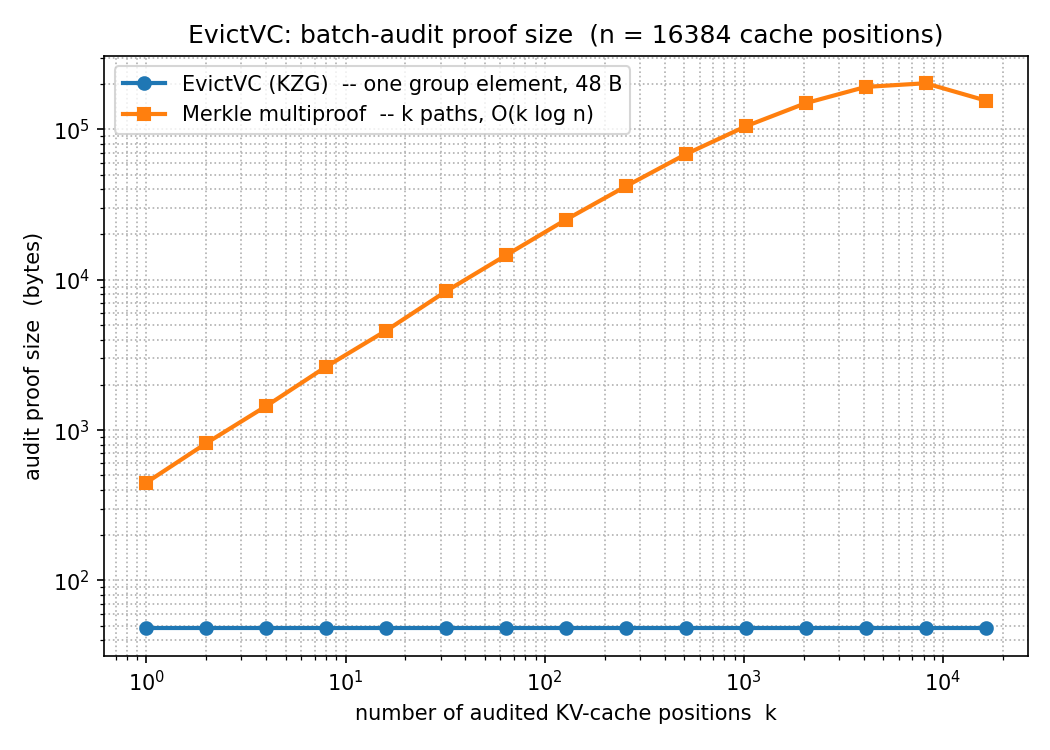
\includegraphics[width=0.72\linewidth]{evictvc_fig1}
\caption{Batch-audit proof size versus number of audited positions $k$
($n=2^{14}$). EvictVC's proof is a constant $48$-byte group element; the Merkle
multiproof grows with $k$.}
\label{fig:proofsize}
\end{figure}

\subsection{Amortized proof generation}
Table~\ref{tab:fk} contrasts the Feist--Khovratovich all-proofs routine with the
naive baseline of computing one opening per position. The two scale differently
in the most consequential way. Naively, a single opening costs $O(n\log n)$, so
producing a proof for every position costs $O(n^2\log n)$; the ``naive all''
column is simply $n$ times the measured single-open cost. Feist--Khovratovich
instead obtains all $n$ proofs from one $O(n\log n)$ group-FFT pass, an
$O(\log n)$ amortized cost per position. This shows up in the table as a
qualitative difference in the per-proof trend: FK's amortized cost creeps only
from $3.1$ to $4.7\,$ms across $2^8$ to $2^{12}$ (a logarithmic drift), while the
naive single-open cost climbs roughly linearly ($6$ to $59\,$ms over the same
window). The crossover is immediate---at every measured size FK's amortized
per-proof already undercuts a single naive opening (at $2^{12}$, $4.7\,$ms versus
$59\,$ms, a $12\times$ gap)---and the ratio widens with $n$.

At full-cache scale the separation becomes decisive. A single opening at
$n=2^{16}$ costs ${\approx}\,684\,$ms (Table~\ref{tab:maint}), so producing all
$2^{16}$ proofs naively would take
$684\,\text{ms}\times2^{16}\approx 4.5\times10^{4}\,$s, about $12.5$ hours; the FK
routine, extrapolating its $O(n\log n)$ trend, completes the same task in roughly
$7$ minutes single-threaded, and its FFT parallelizes cleanly across cores.
Beyond a handful of openings, FK is therefore not merely faster but the only
feasible way to serve whole-cache audits. One honest caveat: FK's absolute
per-proof cost is milliseconds, not microseconds, because the group-FFT performs
$O(n\log n)$ scalar multiplications by roots of unity; the win is the asymptotic
$O(n\log n)$-versus-$O(n^2)$ separation in total work---realized here as hours
versus minutes---rather than a small per-proof constant.

\begin{table}[t]\centering
\renewcommand{\arraystretch}{1.1}
\begin{tabular}{@{}rrrrr@{}}
\toprule
$n$ & FK all (ms) & FK / proof ($\mu s$) & naive open (ms) & naive all (est., s)\\
\midrule
$2^{8}$  & $800.7$   & $3127.8$ & $6.13$  & $1.6$\\
$2^{10}$ & $3980.3$  & $3887.0$ & $18.32$ & $18.8$\\
$2^{12}$ & $19095.5$ & $4662.0$ & $59.21$ & $242.5$\\
\bottomrule
\end{tabular}
\caption{Feist--Khovratovich all-proofs versus naive per-position opening
(BLS12-381, single thread). FK's amortized per-proof cost grows only
logarithmically; the naive all-proofs estimate is $n\times$ a single opening.}
\label{tab:fk}
\end{table}

\paragraph{Summary.}
The three measurements validate the design end-to-end and along independent axes.
Constant-time eviction (Table~\ref{tab:maint}) makes it practical to apply the
commitment per evicted token in a streaming compressor, where the cache is
rewritten continuously. Constant-size, aggregatable audits
(Figure~\ref{fig:proofsize}) make verification scale \emph{in} the number of
checked positions rather than against it, so an auditor can sample as
aggressively as it likes for a fixed $48$-byte proof and two pairings. And
amortized proof generation (Table~\ref{tab:fk}) makes serving openings for the
entire, possibly-evicted cache feasible at a scale where the naive approach is
hours out of reach. None of these rests on a faster primitive than the
alternatives in isolation; each follows from the algebraic structure---homomorphic
$O(1)$ updates, one-element subvector openings, and batched proof
computation---that the KZG instantiation provides and a hash-based commitment does
not.

% =====================================================================
\section{Conclusion}\label{sec:conc}
% =====================================================================

We introduced evictable vector commitments, a primitive that brings permanent,
policy-checked deletion---with a tamper-evident history---to the vector
commitments underlying verifiable LLM inference, and gave a KZG construction with
$O(1)$ eviction, single-element batch-audit proofs, and quasi-linear all-proof
maintenance, proven secure under $\nsdh$ and collision resistance.

Several extensions are natural. \emph{Set-relative policies} such as
$\arg\min$/bottom-$k$ eviction require a verifiable minimality or sorting argument
over the committed score vector, layered on the threshold policy proven here.
\emph{Succinct history membership} would let an auditor prove a single past
eviction without replaying the whole log, e.g.\ by replacing the hash chain with
a Merkle Mountain Range. \emph{Confidential eviction} could hide the evicted
values---revealing only their commitments and update proofs---when the dropped
state is sensitive. Finally, integrating EvictVC into an end-to-end
verifiable-inference pipeline over a real streaming KV-cache compressor is the
natural systems follow-up.

% =====================================================================
% Bibliography. Verify final page numbers against CryptoBib
% (https://cryptobib.di.ens.fr/) before camera-ready.
% =====================================================================
\begin{thebibliography}{99}
\bibitem{kzg} A.~Kate, G.~M.~Zaverucha, and I.~Goldberg.
  \emph{Constant-Size Commitments to Polynomials and Their Applications.}
  ASIACRYPT 2010, LNCS vol.~6477, pp.~177--194. Springer, 2010.
\bibitem{fk} D.~Feist and D.~Khovratovich.
  \emph{Fast Amortized Kate Proofs.} Ethereum Research, 2020.
\bibitem{cf13} D.~Catalano and D.~Fiore.
  \emph{Vector Commitments and Their Applications.} PKC 2013, LNCS vol.~7778,
  pp.~55--72. Springer, 2013.
\bibitem{tomescu} A.~Tomescu, I.~Abraham, V.~Buterin, J.~Drake, D.~Feist, and
  D.~Khovratovich. \emph{Aggregatable Subvector Commitments for Stateless
  Cryptocurrencies.} SCN 2020, LNCS vol.~12238, pp.~45--64. Springer, 2020.
\bibitem{streamingllm} G.~Xiao, Y.~Tian, B.~Chen, S.~Han, and M.~Lewis.
  \emph{Efficient Streaming Language Models with Attention Sinks.}
  ICLR 2024. arXiv:2309.17453.
\bibitem{h2o} Z.~Zhang, Y.~Sheng, T.~Zhou, T.~Chen, L.~Zheng, R.~Cai, Z.~Song,
  Y.~Tian, C.~R\'e, C.~Barrett, et al.
  \emph{H2O: Heavy-Hitter Oracle for Efficient Generative Inference of Large
  Language Models.} NeurIPS 2023.
\bibitem{snapkv} Y.~Li, Y.~Huang, B.~Yang, et al.
  \emph{SnapKV: LLM Knows What You Are Looking For Before Generation.}
  NeurIPS 2024.
\bibitem{zkllm} H.~Sun, J.~Li, and H.~Zhang.
  \emph{zkLLM: Zero Knowledge Proofs for Large Language Models.}
  ACM CCS 2024, pp.~4405--4419. arXiv:2404.16109.
\bibitem{verillm} K.~Wang et al.
  \emph{VeriLLM: A Lightweight Framework for Publicly Verifiable Decentralized
  Inference.} arXiv:2509.24257, 2025.
\bibitem{svip} Y.~Sun, Y.~Li, Y.~Zhang, Y.~Jin, and H.~Zhang.
  \emph{SVIP: Towards Verifiable Inference of Open-Source Large Language Models.}
  arXiv:2410.22307, 2025.
\bibitem{toploc} J.~M.~Ong, M.~Di~Ferrante, A.~Pazdera, R.~Garner, S.~Jaghouar,
  M.~Basra, M.~Ryabinin, and J.~Hagemann.
  \emph{TopLoc: A Locality-Sensitive Hashing Scheme for Trustless Verifiable
  Inference.} arXiv, 2025.
\end{thebibliography}

\end{document}
